%%%%%%%%%%%%%%%%%%%%%%%%%%%%%%%%%%%%%%%%%%%%%%%%%%%%%%%%%%%%%%%%%%%%%%%%%%%%%%
\subsection{DAQ}
Top view of the DAQ configuration hierarchy is shown in Figure~\ref{figure:daq_config}.

\begin{figure}[H]
  \begin{tikzpicture}
    \node[anchor=south west,inner sep=0] at (0,0.) {
      % \node[shift={(0 cm,0.cm)},inner sep=0,rotate={90}] at (0,0) {}
      \makebox[\textwidth][c] {
        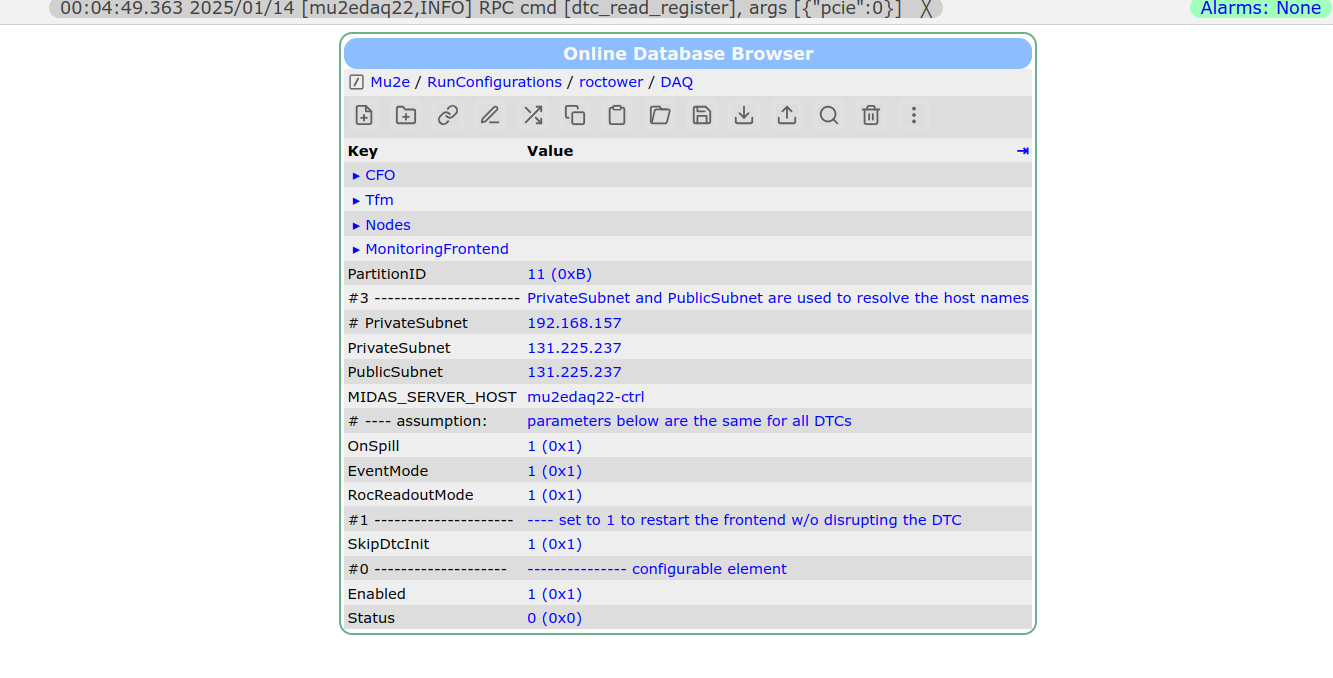
\includegraphics[width=0.95\textwidth]{png/daq_configuration}
      }
    };
    % \node [text width=8cm, scale=1.0] at (14.5,0.5) {$\mu_B$, expected background mean};
    % \node [text width=8cm, scale=1.0, rotate={90}] at (1.5,7.5) { $S_{D}$, ``discovery'' signal strength  };
  \end{tikzpicture}
  \caption{
    \label{figure:daq_config}
    Top level of the DAQ configuration
  }
\end{figure}

It includes configuration of the CFO, the Trigger Farm Manager (TRM), configuration
of the trigger farm nodes and a numebr of global DAQ parameters.


%%%%%%%%%%%%%%%%%%%%%%%%%%%%%%%%%%%%%%%%%%%%%%%%%%%%%%%%%%%%%%%%%%%%%%%%%%%%%%
\newpage
\subsubsection{Emulated CFO configuration}
An example of the emulated CFO configuration is shown in Figure~\ref{figure:cfo_config}.
It includes a link to the configuration of the corresponding FPGA (DTC) 
defined within the same configuration, and a list of the CFO-specific parameters.

\begin{figure}[H]
  \begin{tikzpicture}
    \node[anchor=south west,inner sep=0] at (0,0.) {
      % \node[shift={(0 cm,0.cm)},inner sep=0,rotate={90}] at (0,0) {}
      \makebox[\textwidth][c] {
        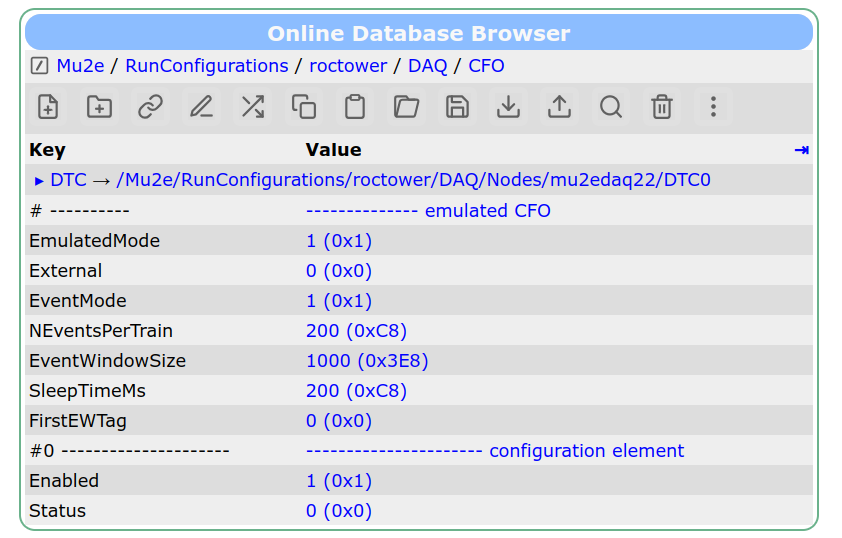
\includegraphics[width=0.95\textwidth]{png/cfo_configuration}
      }
    };
    % \node [text width=8cm, scale=1.0] at (14.5,0.5) {$\mu_B$, expected background mean};
    % \node [text width=8cm, scale=1.0, rotate={90}] at (1.5,7.5) { $S_{D}$, ``discovery'' signal strength  };
  \end{tikzpicture}
  \caption{
    \label{figure:cfo_config}
    CFO configuration
  }
\end{figure}

%%%%%%%%%%%%%%%%%%%%%%%%%%%%%%%%%%%%%%%%%%%%%%%%%%%%%%%%%%%%%%%%%%%%%%%%%%%%%%
\newpage
\subsubsection{Hardware CFO configuration}

\add{To be added}

% \begin{figure}[H]
%   \begin{tikzpicture}
%     \node[anchor=south west,inner sep=0] at (0,0.) {
%       % \node[shift={(0 cm,0.cm)},inner sep=0,rotate={90}] at (0,0) {}
%       \makebox[\textwidth][c] {
%         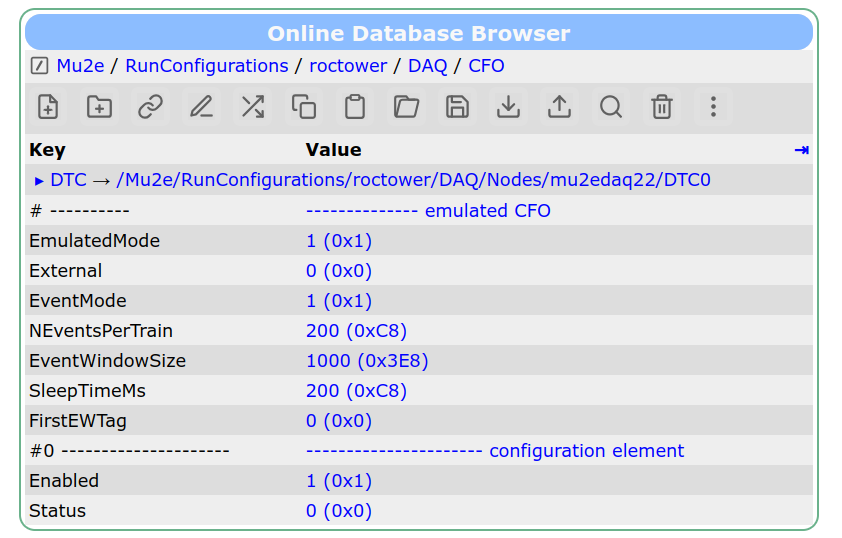
\includegraphics[width=0.95\textwidth]{png/cfo_configuration}
%       }
%     };
%     % \node [text width=8cm, scale=1.0] at (14.5,0.5) {$\mu_B$, expected background mean};
%     % \node [text width=8cm, scale=1.0, rotate={90}] at (1.5,7.5) { $S_{D}$, ``discovery'' signal strength  };
%   \end{tikzpicture}
%   \caption{
%     \label{figure:cfo_config}
%     CFO configuration
%   }
% \end{figure}
% 

%%%%%%%%%%%%%%%%%%%%%%%%%%%%%%%%%%%%%%%%%%%%%%%%%%%%%%%%%%%%%%%%%%%%%%%%%%%%%%
\subsubsection{DAQ-specific frontends}

\begin{itemize}
\item
  one monitoring/control frontend per DAQ server. Monitoring:
  \begin{itemize}
  \item
    2 DTC's with 6 ROCs per DTC
  \item
    ARTDAQ processes:
    \begin{itemize}
    \item
      2 boardreaders, N event builders, potentially a data logger, and a dispatcher
    \end{itemize}
  \item
    overall health: amount of free space available
  \end{itemize}
\item
  emulated CFO:
  \begin{itemize}
  \item
    currently : a separate frontend 
  \item 
    make the CFO frontend a separate thread of the node frontend
  \end{itemize}
\item
  external CFO frontend 
\item
  global control frontend:
\end{itemize}

%%%%%%%%%%%%%%%%%%%%%%%%%%%%%%%%%%%%%%%%%%%%%%%%%%%%%%%%%%%%%%%%%%%%%%%%%%%%%%
\subsection{ARTDAQ configuration}

ARTDAQ configuration is stored in ODB. It consists of two parts:
\begin{itemize}
\item
  Trigger Farm Manager (TFM) configuration
\item
  configuration of the artdaq processes on each farm node
\end{itemize}

A configuration of a single node is shown in Figure ~\ref{figure:artdaq_configuration}.

\begin{figure}[H]
  \begin{tikzpicture}
    \node[anchor=south west,inner sep=0] at (0,0.) {
      % \node[shift={(0 cm,0.cm)},inner sep=0,rotate={90}] at (0,0) {}
      \makebox[\textwidth][c] {
        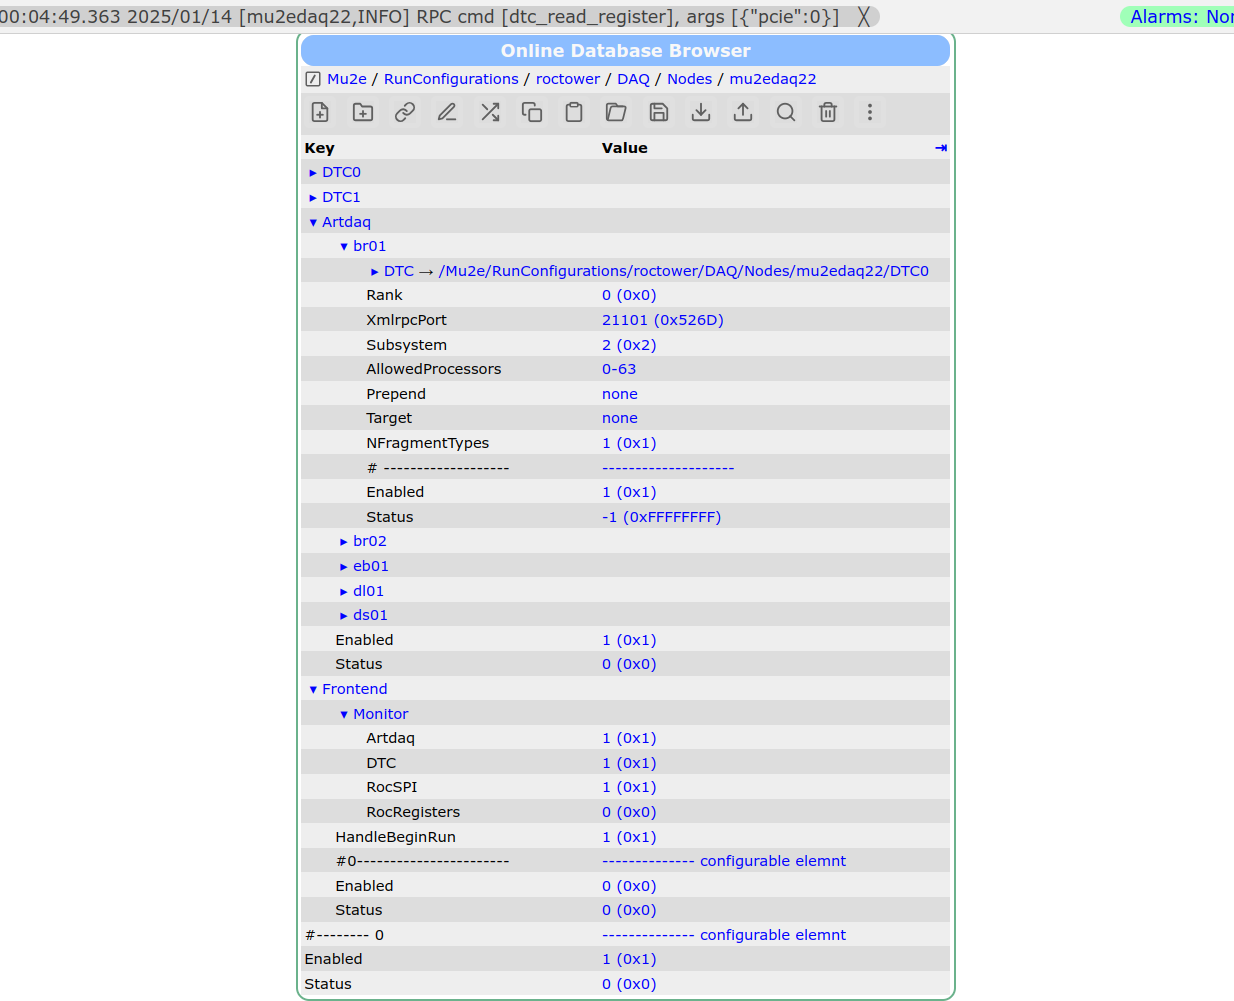
\includegraphics[width=0.95\textwidth]{png/artdaq_configuration}
      }
    };
    % \node [text width=8cm, scale=1.0] at (14.5,0.5) {$\mu_B$, expected background mean};
    % \node [text width=8cm, scale=1.0, rotate={90}] at (1.5,7.5) { $S_{D}$, ``discovery'' signal strength  };
  \end{tikzpicture}
  \caption{
    \label{figure:artdaq_configuration}
    CFO configuration
  }
\end{figure}

It has
\begin{itemize}
\item
  parameters of the DTCs. There could be zero, one, or two DTCs on a farm node.
\item
  parameters of the artdaq processes running on that node.
  Configuration of the ARTDAQ boardreaders has links to the definitions
  of the DTCs they are reading. A boardreader need to know the PCIE address of the DTC
  it is interacting with. At start time, the boardreaders query that information
  from the ODB.
  
\item
  parameters of the node control frontend, including the configuration of the
  slow controls ("Frontend/Monitor")
\end{itemize}

%%%%%%%%%%%%%%%%%%%%%%%%%%%%%%%%%%%%%%%%%%%%%%%%%%%%%%%%%%%%%%%%%%%%%%%%%%%%%%
\subsection{DAQ-to-subdetectors interface}
The DAQ elements are "mapped" linked to the corresponding subdetector elements using ODB links,
as shown in Figure ~\ref{figure:daq_to_tracker_interface}.
\begin{figure}[H]
  \begin{tikzpicture}
    \node[anchor=south west,inner sep=0] at (0,0.) {
      % \node[shift={(0 cm,0.cm)},inner sep=0,rotate={90}] at (0,0) {}
      \makebox[\textwidth][c] {
        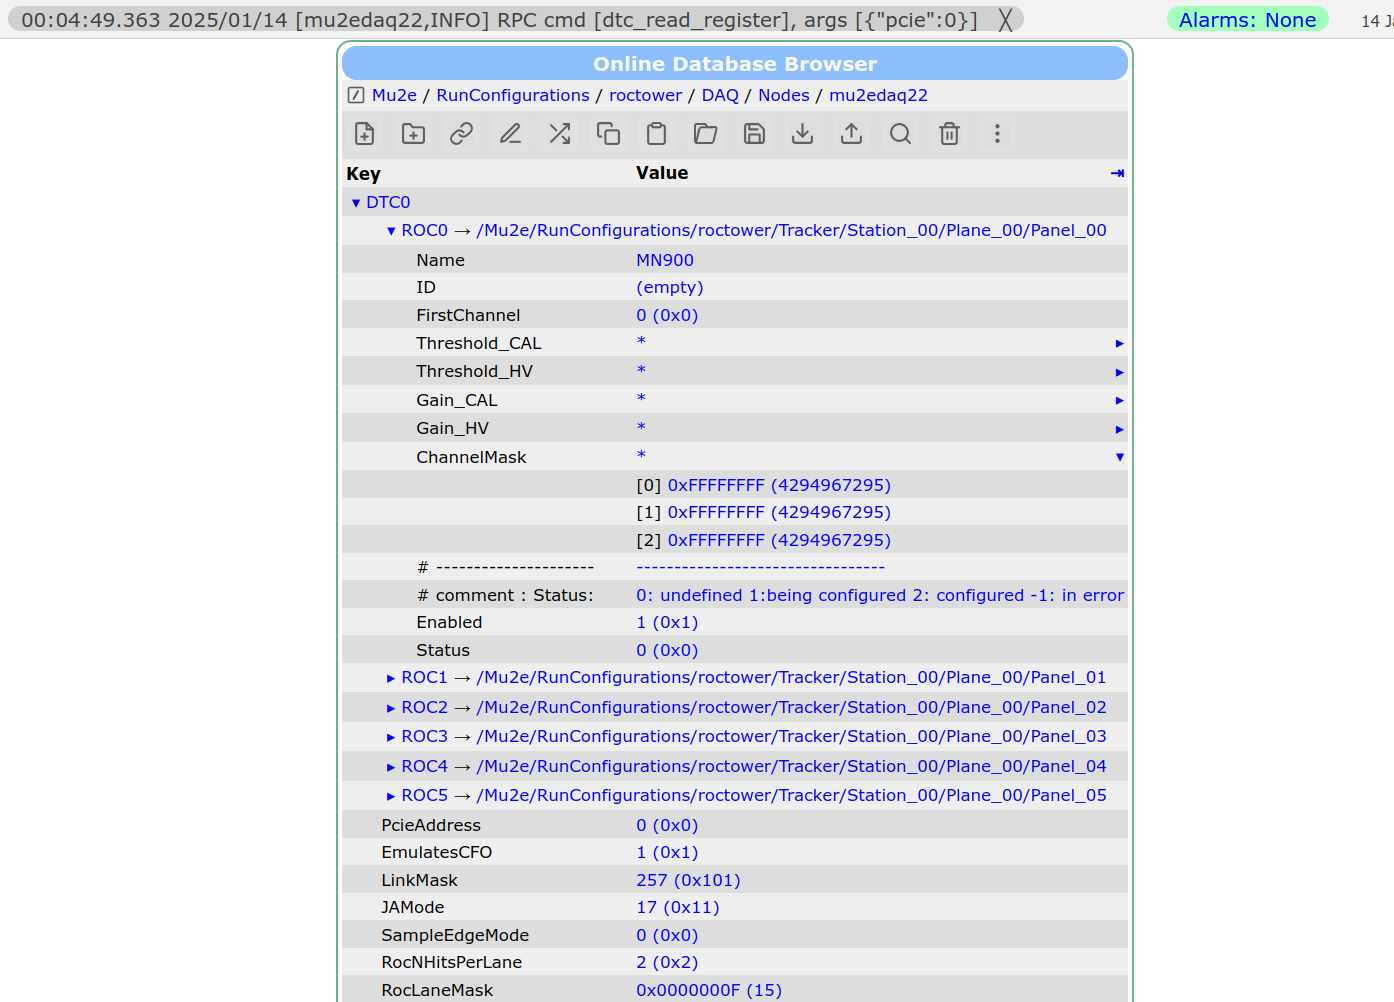
\includegraphics[width=0.95\textwidth]{png/daq_to_tracker_interface}
      }
    };
    % \node [text width=8cm, scale=1.0] at (14.5,0.5) {$\mu_B$, expected background mean};
    % \node [text width=8cm, scale=1.0, rotate={90}] at (1.5,7.5) { $S_{D}$, ``discovery'' signal strength  };
  \end{tikzpicture}
  \caption{
    \label{figure:daq_to_tracker_interface}
    CFO configuration
  }
\end{figure}

A DAQ node has links to the DTCs installed on that node, and the tracker DTC ROCs shown have
links to the definitions of the tracker panels they are reading.

%%% Local Variables:
%%% mode: latex
%%% TeX-master: t
%%% End:
